\documentclass{beamer}
\RequirePackage{preamble}

\title{Presentatie KMA}
\date[26-03-2024]{March 26th, 2024}
\author[Danny Blom]{Danny Blom}

\usetheme{kep}

\newcommand{\hospitals}{\mathcal{H}}
\newcommand{\exchanges}{\mathcal{E}}

\begin{document}
              
\begin{frame}
    \maketitle 
\end{frame}

\begin{frame}{Kidney exchange}
    \begin{figure}
    \tikzset{cross/.style={cross out, draw=red, fill=none, minimum size=2*(#1-\pgflinewidth), inner sep=0pt, outer sep=0pt}, cross/.default={2pt}}
    \centering
    \begin{tikzpicture}[overlay, remember picture]
        \tikzstyle{arc}=[-stealth, very thick, shorten >=2pt, shorten <=2pt];
        \tikzstyle{vertex}=[circle, draw=blue, fill=blue!30];
    
        % HENK EN INGRID
        \onslide<+->{
            \node[label=below:Patient $A$] (henk) at ($(current page.north)+(-3,-2.5)$) {
\includegraphics[width=2cm, height=2cm]{./Figures/Pictures/henk.png}};
            \node[label=below:Donor $A$] (ingrid) at ($(current page.north)+(1,-2.5)$) {
\includegraphics[width=2cm, height=2cm]{./Figures/Pictures/ingrid.png}};
            \node (space) at ($(ingrid.east)+(4,0)$) {.};
            }
    
        \draw<+>[arc] (ingrid.west) -- node[midway] {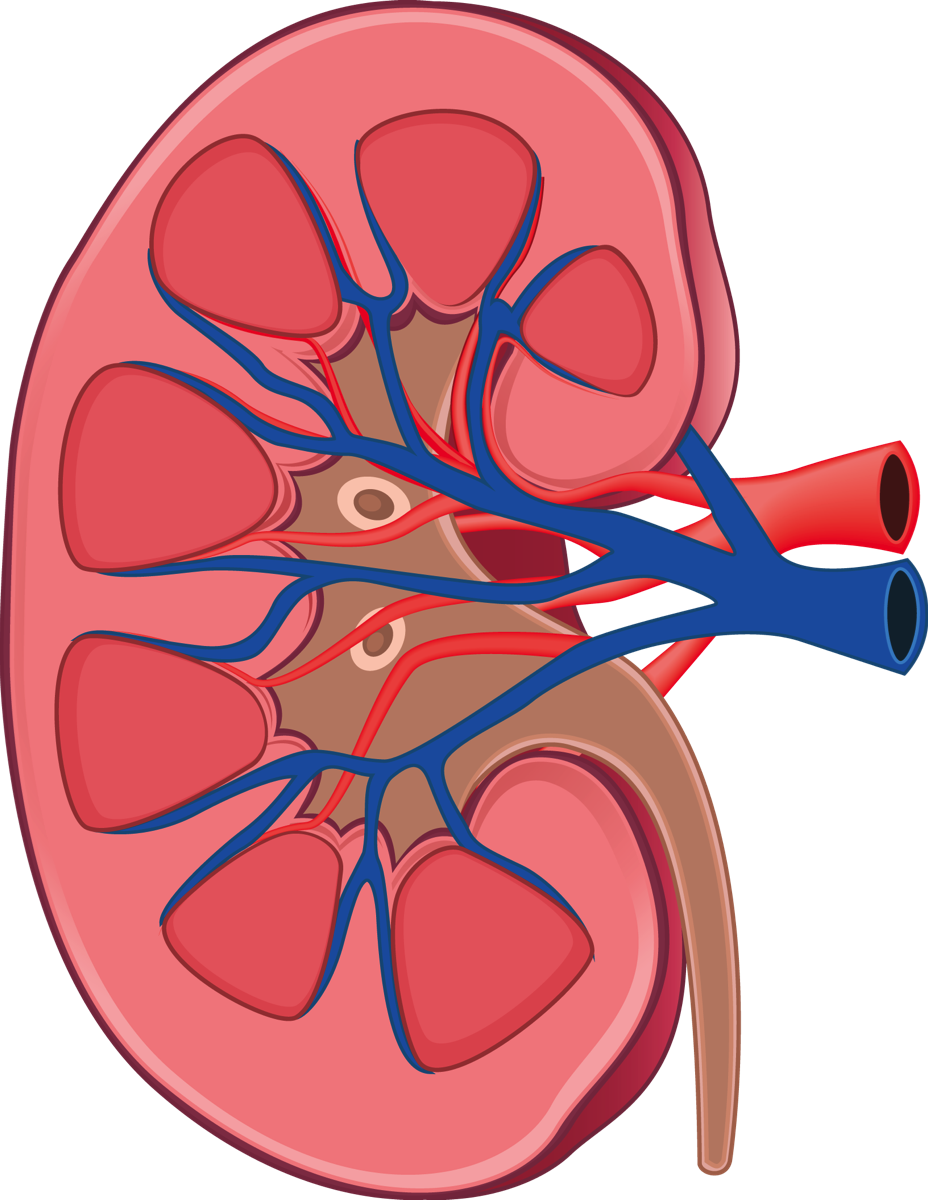
\includegraphics[width=10pt]{./Figures/Pictures/kidney.png}} (henk.east);
        
        \onslide<+->{
            \draw[arc, red] (ingrid.west) -- (henk.east);
            \draw ($(ingrid.west)!.5!(henk.east)$) node[cross=5pt, ultra thick] {};
        }
    
        % AHMED EN FATIMA
        \onslide<+->{
            \node[label=below:Patient $B$] (fatima) at ($(current page.north)+(-3,-5.5)$) {
\includegraphics[width=2cm, height=2cm]{Figures/Pictures/fatima.png}};
            \node[label=below:Donor $B$] (ahmed) at ($(current page.north)+(1,-5.5)$) {
\includegraphics[width=2cm, height=2cm]{Figures/Pictures/ahmed.png}};
        }
    
        \draw<+>[arc] (ahmed.west) -- node[midway] {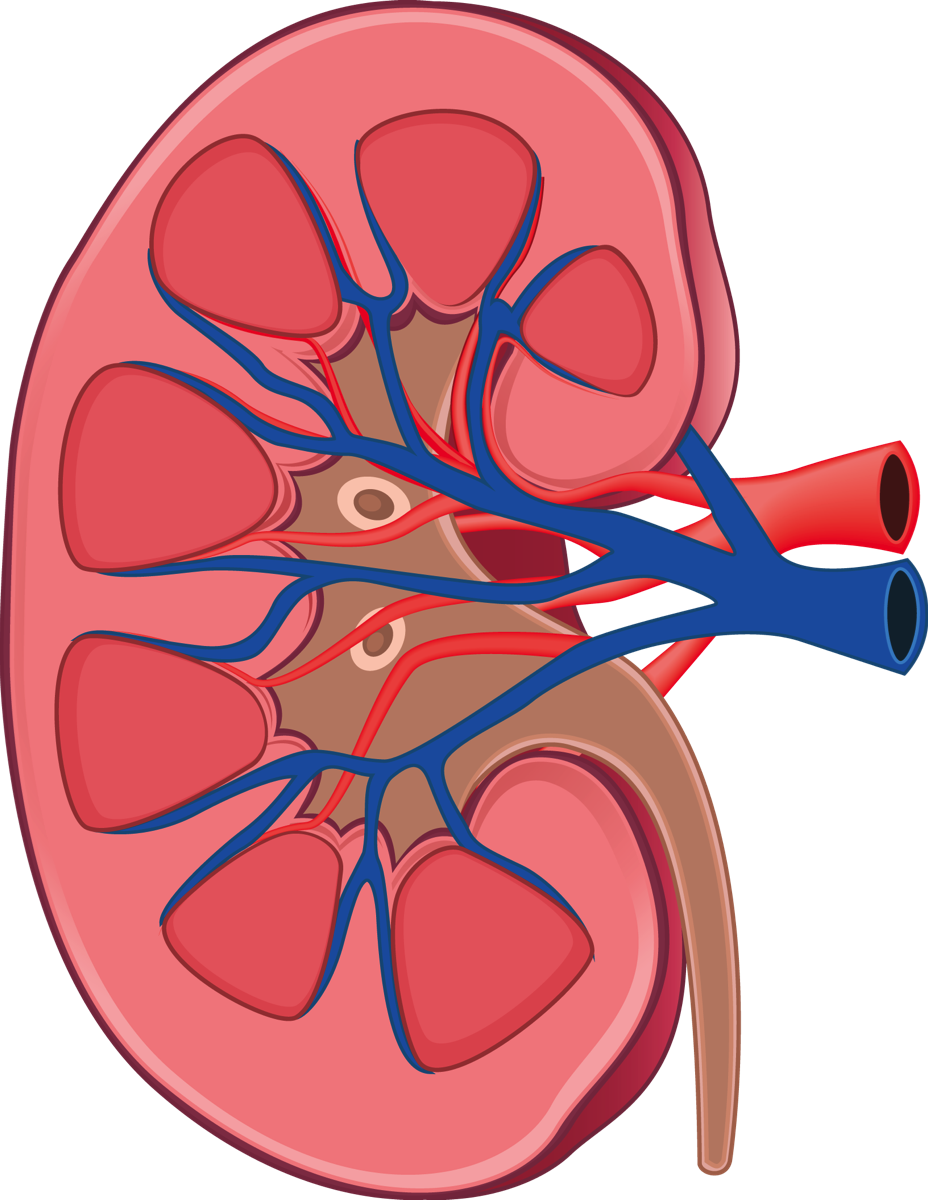
\includegraphics[width=10pt]{./Figures/Pictures/kidney.png}} (fatima.east);
        
        \onslide<+->{
            \draw[arc, red] (ahmed.west) -- (fatima.east);
            \draw ($(ahmed.west)!.5!(fatima.east)$) node[cross=5pt, ultra thick] {};
        }
    
        \onslide<+->{
            \draw[arc, green] (ahmed.160) -- node[pos=0.25, sloped]{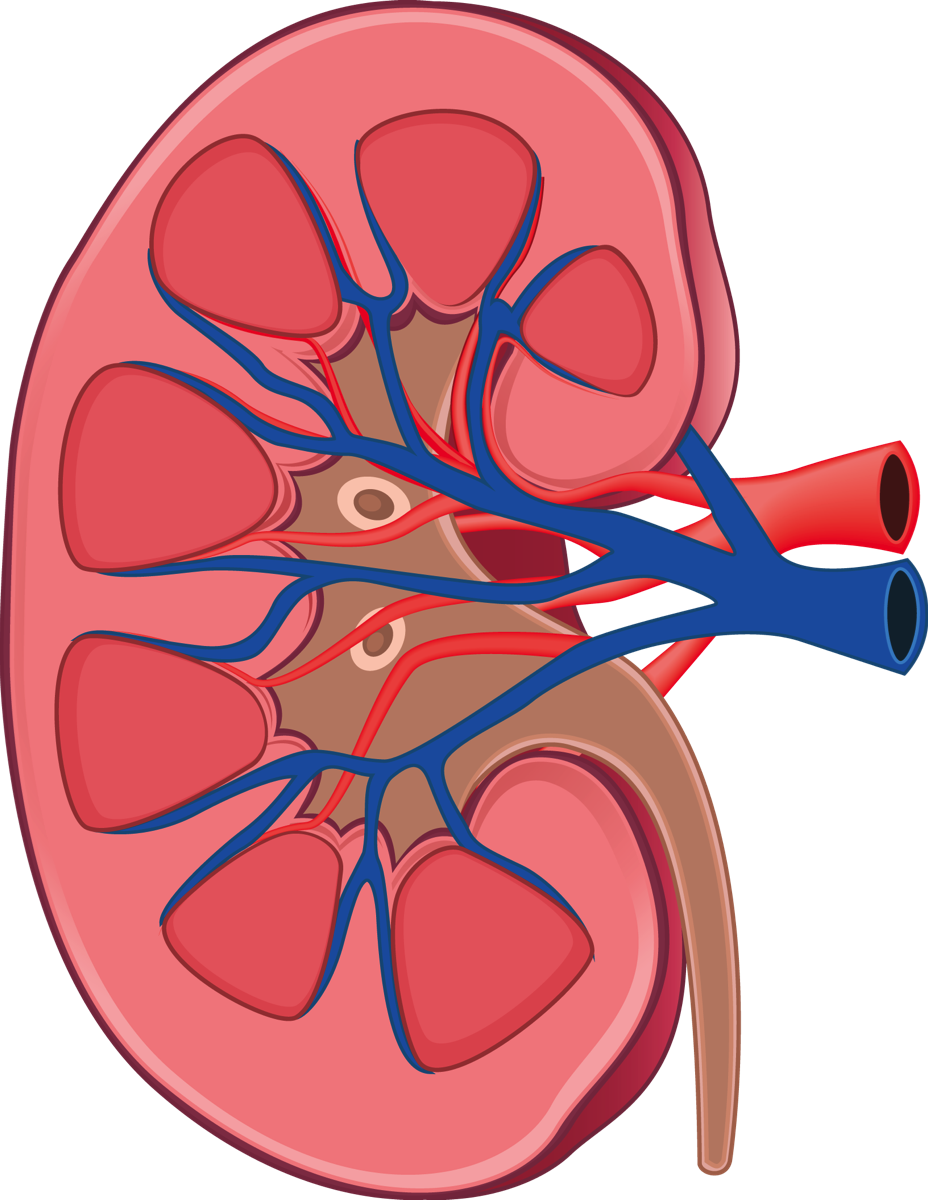
\includegraphics[width=10pt]{./Figures/Pictures/kidney.png}} (henk.320);
            \draw[arc, green] (ingrid.200) -- node[pos=0.25, sloped]{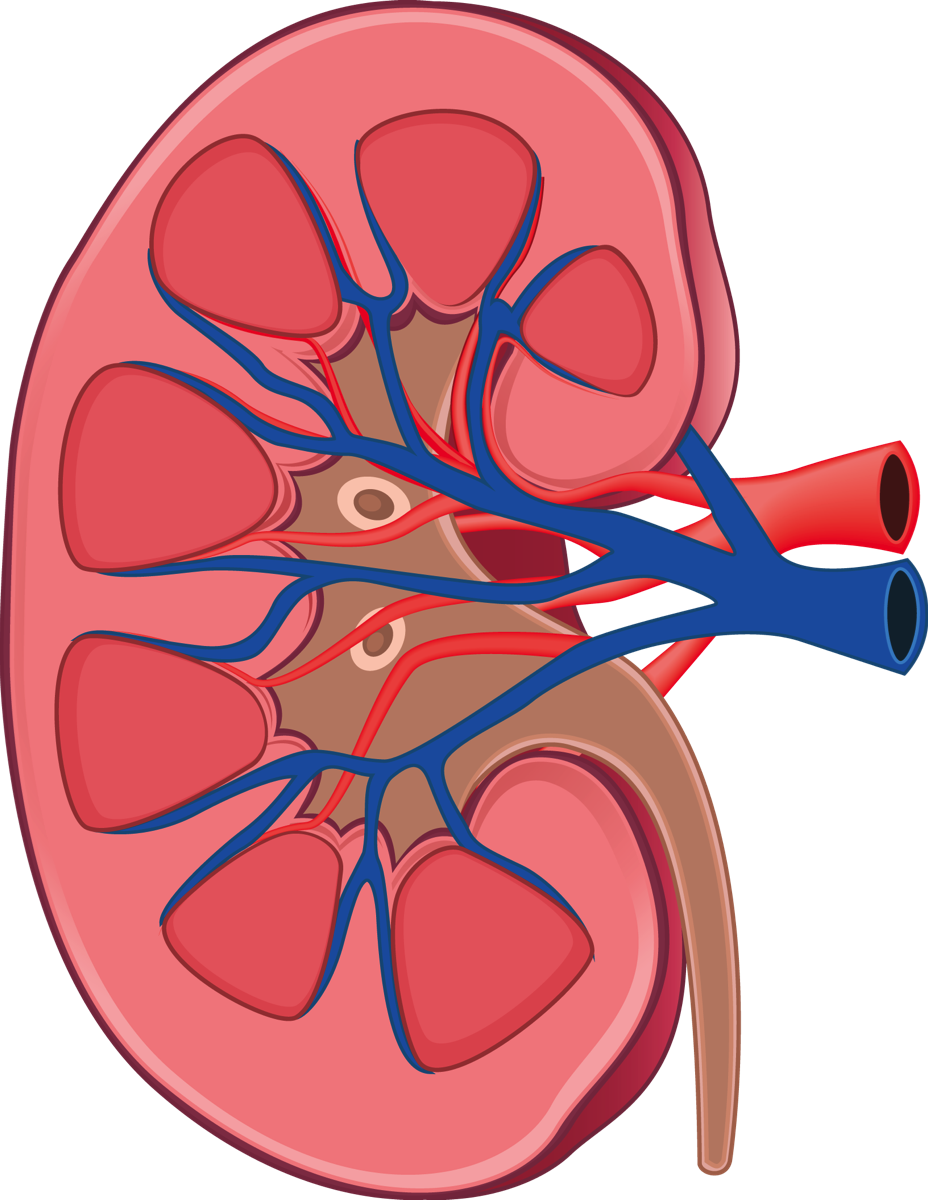
\includegraphics[width=10pt]{./Figures/Pictures/kidney.png}} (fatima.40);
        }
    
        \onslide<+->{
            \node[vertex, label=90:{$p_{A} = (r_{A}, d_{A})$}] (pairhi) at ($(ingrid.east)+(2,0)$) {};
            
            \node[vertex, label=270:{$p_{B} = (r_{B}, d_{B})$}] (pairfa) at ($(ahmed.east)+(2,0)$) {};
    
            \draw[arc, bend right=20] (pairhi.south west) to (pairfa.north west);
            \draw[arc, bend right=20] (pairfa.north east) to (pairhi.south east);
            
        }
    \end{tikzpicture}

\end{figure}

    \vskip6cm%
    \onslide<+->{
        Hoe kies je `exchanges' om het aantal transplantaties te maximaliseren?
    }
\end{frame}

\begin{frame}{Een breed en divers onderzoeksveld}
    \begin{center}
    \begin{tikzpicture}[remember picture]
        \tikzstyle{vertex} = [cloud, draw=black, fill=gray!30, aspect=2.4, inner sep=0pt, align=center];
            
        % Draw instance with proposed solution
        \onslide<1->{
            \node[vertex, align=center] (v1) at ($(current page.north)+(-7,-2)$) {\small\begin{tabular}{c} Mixed-integer \\ linear programming \end{tabular}};
            \node[vertex, align=center] (v2) at ($(current page.north)+(-3,-4.5)$) {\small Samenwerkingen};
            \node[vertex, align=center] (v3) at ($(current page.north)+(-7.5,-5)$) {\small\begin{tabular}{c} Optimalisatie \\ met \\ onzekerheid \end{tabular}};
            \node[vertex, align=center] (v4) at ($(current page.north)+(-.5,-2.5)$) {\small\begin{tabular}{c} Cross-match \\ tests \end{tabular}};
            \node[vertex, align=center] (v5) at ($(current page.north)+(-4,-7)$) {\small\begin{tabular}{c} Multi-objective \\ optimization \end{tabular}};
            \node[vertex, align=center, inner sep=5pt] (v6) at ($(current page.north)+(0.5,-5.5)$) {\small Ethiek};
    		\node[vertex, align=center, inner sep=7pt] (v7) at ($(current page.north)+(-3,-1.5)$) {\small...};
    		\node[vertex, align=center, inner sep=10pt] (v8) at ($(current page.north)+(-8,-7.5)$) {...};
    		\node[vertex, align=center, inner sep=10pt] (v9) at ($(current page.north)+(0,-7.5)$) {...};       
    	}

        \onslide<2->{
            \node[vertex, fill=blue!30] (v7) at ($(current page.north)+(-3,-4.5)$) {\small Samenwerkingen};
        }

    \end{tikzpicture}
\end{center}

\end{frame}

\begin{frame}{Samenwerkingen in kidney exchange}
\vspace{-3cm}%
\textbf{Realiteit:} veel \emph{kidney exchange programmas} worden door een individueel ziekenhuis / transplantatiecentrum beheerd.
\vskip5pt%

\onslide<4->{
    \textbf{Idee: } samenvoegen van pools van verschillende programma's!
}

\onslide<2->
{

    \vskip10pt%
    \begin{figure}
    \centering
    \begin{tikzpicture}[overlay, remember picture,scale=0.9]
        \tikzstyle{arc}=[-stealth, dashed, thin, shorten >=2pt, shorten <=2pt];
        \tikzstyle{arcbend}=[arc, bend right=10];
        \tikzstyle{usedarc}=[arc, solid, very thick];
        \tikzstyle{usedarcbend}=[usedarc, bend right=10];
        
        \tikzstyle{bluenode}=[draw=blue, fill=blue!30, circle];
        \tikzstyle{rednode}=[draw=red, fill=red!30, circle];
        
        % BLUE AND RED VERTICES, AND INTERNAL ARCS
        \node (bluehospital) at (-2, 0) {
\includegraphics[scale=0.8]{Figures/Pictures/blue_hospital.pdf}};
        \node[right of=bluehospital] (redhospital) at (2,0) {
\includegraphics[scale=0.8]{Figures/Pictures/red_hospital.pdf}};
        
        \foreach \i in {1,2,3}
        {
            \node[bluenode, label=225:{$p_{\i}$}] (v\i) at ($(bluehospital)-(0,3)+(-120+120*\i:1.5cm)$) {};
        }

        \foreach \i [count=\x] in {A,B,C,D}
        {
            \pgfmathsetmacro\location{int(45+90*(\x-1))}
            \node[rednode, label=\location:{$p_{\i}$}] (v\i) at ($(redhospital)-(0,3)+(-45+90*\x:1.5cm)$) {};
        }      
        
        \foreach \i/\j in {A/B, B/D, C/B}
            \draw[arc] (v\i) to (v\j);
        
        \foreach \i/\j in {1/2, 2/1, 2/3, 3/2, A/D, D/A}
            \draw[arcbend] (v\i) to (v\j);
        
        % DRAW SOLUTION
        \onslide<3>{
            \foreach \i/\j in {C/B}
                \draw[arc] (v\i) to (v\j);
            
            \foreach \i/\j in {A/B, B/D}
                \draw[usedarc] (v\i) to (v\j);
            
            \foreach \i/\j in {2/3, 3/2, A/D}
                \draw[arcbend] (v\i) to (v\j);
       
            \foreach \i/\j in {1/2, 2/1, D/A}
                \draw[usedarcbend] (v\i) to (v\j);
        }

        % DRAW INTERNATIONAL ARCS
        \onslide<4>{
            \foreach \i/\j in {A/B, B/D, C/B}
                \draw[arc] (v\i) to (v\j);
            
            \foreach \i/\j in {}
                \draw[usedarc] (v\i) to (v\j);
            
            \foreach \i/\j in {1/2, 2/1, 2/3, 3/2, A/D, D/A}
                \draw[arcbend] (v\i) to (v\j);
       
            \foreach \i/\j in {}
                \draw[usedarcbend] (v\i) to (v\j);

            \foreach \i/\j in {B/1, 1/C, 3/C}
                \draw[arc, purple!90] (v\i) to (v\j);

            % Arrows between hospitals
            \draw[-stealth, very thick] ($(bluehospital.east)-(0,0.2)$) to ($(redhospital.west)-(0,0.2)$);
            \draw[-stealth, very thick] ($(redhospital.west)-(0,.4)$) to ($(bluehospital.east)-(0,.4)$);
        }

        % DRAW MULTI-AGENT KEP SOLUTION
        \onslide<5>{
            \foreach \i/\j in {A/B, B/D}
            {
                \draw[arc] (v\i) to (v\j);
            }
            
            \foreach \i/\j in {B/1, 1/C, C/B}
            {
                \draw[usedarc] (v\i) to (v\j);
            }
            
            \foreach \i/\j in {1/2, 2/1}
            {
                \draw[arcbend] (v\i) to (v\j);
            }
            
            \foreach \i/\j in {2/3, 3/2, A/D, D/A}
            {
                \draw[usedarcbend] (v\i) to (v\j);
            }

            \foreach \i/\j in {B/1, 1/C}
            {
                \draw[usedarc, purple!90] (v\i) to (v\j);
            }
            
            \draw[arc, purple!90] (v3) to (vC);

             % Arrows between hospitals
            \draw[-stealth, very thick] ($(bluehospital.east)-(0,0.2)$) to ($(redhospital.west)-(0,0.2)$);
            \draw[-stealth, very thick] ($(redhospital.west)-(0,.4)$) to ($(bluehospital.east)-(0,.4)$);
        }
    
    \end{tikzpicture}
\end{figure}
}

\end{frame}

\begin{frame}{Issues van samengevoegde pools}
	\vspace{1ex}
	\begin{itemize}
		\item Ziekenhuizen hebben conflicterende doelen
		\begin{itemize}
			\item bv., voornamelijk ge\"interesseerd in hun eigen pati\"enten
		\end{itemize}
		\item Mogelijk minder transplantaties voor een ziekenhuis na samenvoeging
	\end{itemize}
	\vspace{.5cm}
	\begin{enumerate}
		\item Onafhankelijke authoriteit: voorstel van exchanges
		\item Ziekenhuizen: voorstel accepteren / aanpassen
	\end{enumerate}
	
	\begin{figure}
		\centering
		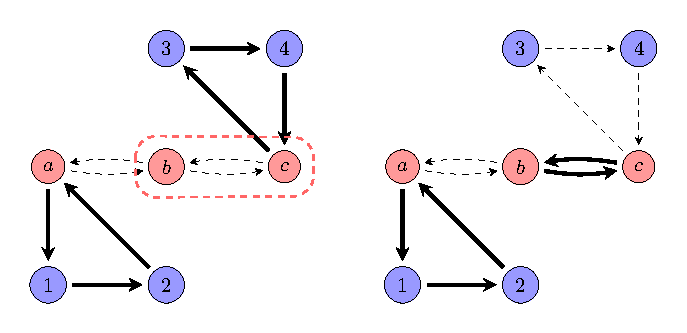
\includegraphics[scale=0.7]{./Figures/Pictures/PartialReject.pdf}
	\end{figure}

\end{frame}

\begin{frame}{Nieuw samenwerkingsmodel}	
\textbf{Idee:} voorstel van exchanges dat ieder ziekenhuis zal accepteren
\vspace{1.5cm}
\begin{enumerate}
	\setlength\itemsep{2em}
	\item Multi-objective optimization
	\begin{enumerate}[(a)]
		\item maximaliseer het aantal transplantaties binnen de pool van ieder ziekenhuis
		\item maximaliseer het totaal aantal transplantaties

	\end{enumerate}
	\item Exact optimization
	\begin{enumerate}[(a)]
		\item maximaliseer het totaal aantal transplant
		\item zodanig dat geen enkel ziekenhuis het voorstel wil aanpassen
	\end{enumerate}
\end{enumerate}
\end{frame}

\begin{frame}{Implementatie \& resultaten}
	\begin{itemize}
		\setlength\itemsep{1em}
		\item Multi-objective optimization
		\begin{itemize}
			\item Losse MILPs voor ieder ziekenhuis
			\item Voeg beperkingen toe die optimaliteit van het primaire doel forceren
		\end{itemize}
		\item Exact optimization: twee-staps optimalisatie
		\begin{itemize}
			\item MIBLP formulering
			\item Cutting plane algoritme op de \emph{high-point relaxation}
		\end{itemize}
		\item Beide algoritmes ge\"implementeerd in C++ / CPLEX
		\item Significant meer transplantaties (tot wel 15\% voor realistische programma's)
		\item Schaalbaar algoritme
	\end{itemize}
\end{frame}

\begin{frame}
    \Huge\centering Vragen? 
\end{frame}

\begin{frame}{Twee-staps optimalisatiemodel}
	\textbf{Parameters:}
	\begin{itemize}
		\item $\hospitals$ \hfill ziekenhuis
		\item $V^{h}$ \hfill incompatibele paren van ziekenhuis $h \in \hospitals$
		\item $\exchanges$ \hfill exchanges
		\item $\exchanges^{h}$ \hfill exchanges binnen de pool van ziekenhuis $h$
		\item $\exchanges^{0}$ \hfill exchanges verspreid over meerdere pools
		\item $w_{e}, w_{e}^{h}$ \hfill waarde van exchange $e$ / voor ziekenhuis $h$
	\end{itemize}
	\vspace{1cm}
	\textbf{Variabelen:}
	\begin{itemize}
		\item $x_{e} \in \{0,1\}$ \hfill OA selecteert exchange $e$ wel of niet?
		\item $y_{e}^{h} \in \{0,1\}$ \hfill Ziekenhuis $h$ selecteert exchange $e$ wel of niet?
	\end{itemize}
\end{frame}

\begin{frame}{Twee-staps optimalisatiemodel}
\vspace{1.5ex}
{\small
	\textbf{Stap 1}
	\begin{align}
		z^{*} = \max_{\vec{x}}~& \sum_{e \in \exchanges} w_{e} x_{e}		 							& \label{obj:upper-level} 				 					\\
		\textrm{s.t.}~& \sum_{e \in \exchanges(v)} y_{e}^{h} 			 \le 1, 					& v \in V \label{con:upper-level:packing} 					\\
		~& \sum_{e \in \exchanges} w_{e}^{h} x_{e} \ge \Phi^{h}(\vec{x}), & h \in \hospitals \label{con:upper-level:shared} \\
		~&y_{e}^{h}	\in \{0,1\}. & e \in \exchanges, h \in \hospitals \label{var:upper-level}										
	\end{align}

	\textbf{Stap 2:}
	\begin{align}
		\Phi^{h}(\vec{x}) = \max_{\vec{y}}~& \sum_{e \in \exchanges} w_{e}^{h} y_{e}^{h} & \label{obj:lower-level} \\
		\textrm{s.t.}~& \sum_{e \in \exchanges(v)} y_{e}^{h} \le 1, & v \in V \label{con:lower-level:packing} \\
		~& y_{e}^{h} \le x_{e}, & e \in \exchanges^{0} \label{con:lower-level:shared} \\
		~&y_{e}^{h}	\in \{0,1\}. & e \in \exchanges, h \in \hospitals \label{var:lower-level}										
	\end{align}
}
	
\end{frame}

\begin{frame}{MILP reformulering}

	$\beta(S^{h})$: \hfill max. waarde van exchanges van de subpool $S^{h} \subseteq V^{h}$
	\vfill\textbf{Reformulering}
	\begin{align}
		z^{*} = \max_{\vec{x}}~& \sum_{e \in \exchanges} w_{e} x_{e} & \label{obj:single-level} \\
		\textrm{s.t.}~& \sum_{e \in \exchanges(v)} x_{e} \le 1, & v \in V \label{con:single-level:packing} 					\\
		~& \sum_{e \in \bigcup\limits_{v \in S^{h}} \exchanges(v)} w_{e}^{h} x_{e} \ge \beta(S^{h}), & h \in \hospitals, S^{h} \subseteq V^{h} \label{con:single-level:subsets} \\
		~&x_{e}	\in \{0,1\}. & e \in \exchanges \label{var:single-level}										
	\end{align}
\end{frame}

\begin{frame}
	\Huge\centering Vragen? 
\end{frame}
\end{document}